\documentclass[tikz,border=5pt]{standalone}
\usepackage{amsmath}
\usepackage[american]{circuitikz}
\usetikzlibrary{arrows.meta,calc}
\definecolor{ink}{HTML}{16324F}
\definecolor{teal}{HTML}{168A88}
\definecolor{gold}{HTML}{D9892B}
\definecolor{redq}{HTML}{B84A4A}
\begin{document}
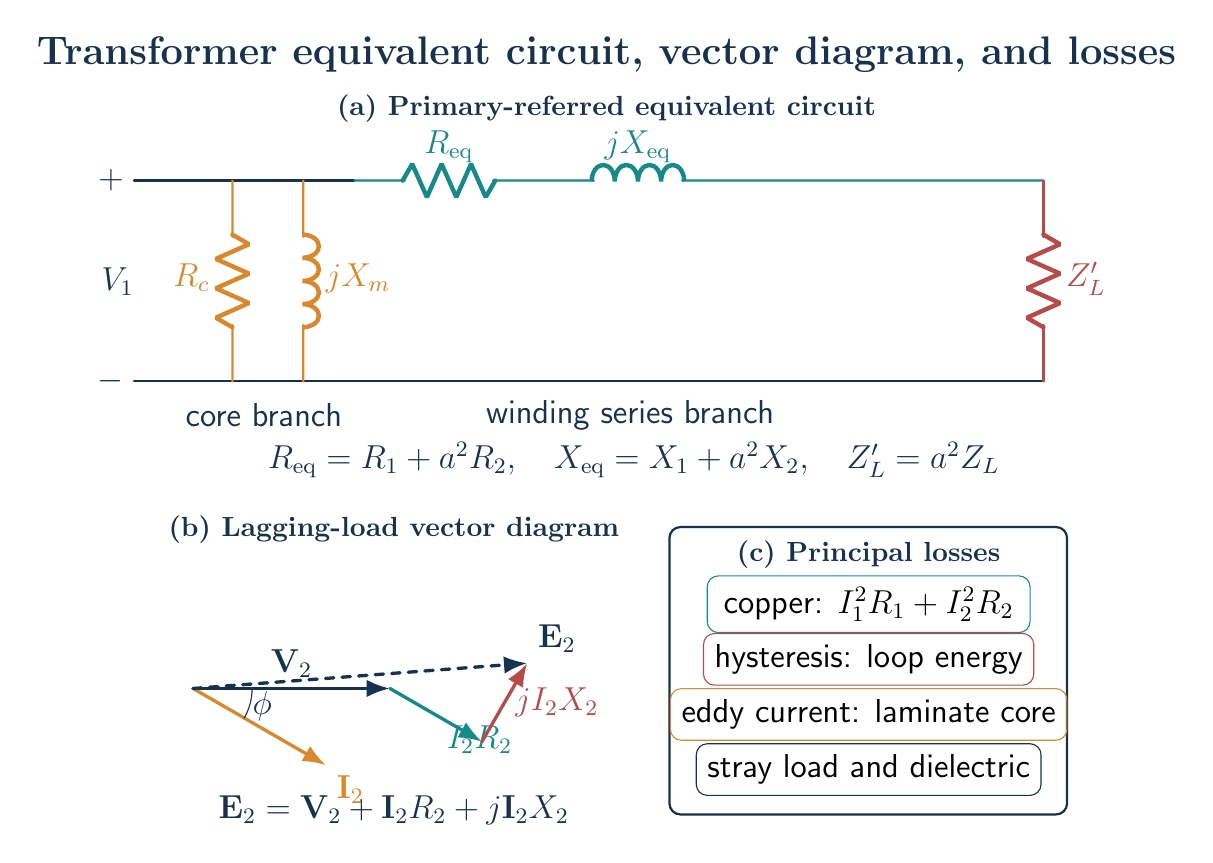
\begin{tikzpicture}[font=\large\sffamily,>=Latex,line cap=round,line join=round]
  \node[font=\bfseries\Large,ink] at (6.25,9.2)
    {Transformer equivalent circuit, vector diagram, and losses};

  \begin{scope}[shift={(.35,4.7)}]
    \node[font=\bfseries,ink] at (5.9,3.82)
      {(a) Primary-referred equivalent circuit};
    \coordinate (T0) at (.35,2.9);
    \coordinate (B0) at (.35,.35);
    \draw[ink,thick] (T0)--(2.7,2.9);
    \draw[ink,thick] (B0)--(11.45,.35);
    \draw[teal,thick] (2.7,2.9) to[R,l=$R_{\rm eq}$] (5.1,2.9)
      to[L,l=$jX_{\rm eq}$] (7.5,2.9)--(11.45,2.9);
    \draw[redq,thick] (11.45,2.9) to[R,l=$Z_L'$] (11.45,.35);
    \draw[gold,thick] (1.15,2.9) to[R,l_=$R_c$] (1.15,.35);
    \draw[gold,thick] (2.05,2.9) to[L,l=$jX_m$] (2.05,.35);
    \draw[ink,thick] (T0)--++(-.45,0) node[left] {\(+\)};
    \draw[ink,thick] (B0)--++(-.45,0) node[left] {\(-\)};
    \node[ink,left] at (.02,1.62) {$V_1$};
    \node[ink] at (1.55,-.08) {core branch};
    \node[ink] at (6.2,-.08) {winding series branch};
    \node[ink,align=center] at (6.25,-.65)
      {$R_{\rm eq}=R_1+a^2R_2,\quad
       X_{\rm eq}=X_1+a^2X_2,\quad Z_L'=a^2Z_L$};
  \end{scope}

  \begin{scope}[shift={(.55,-.55)}]
    \node[font=\bfseries,ink] at (3.0,3.72) {(b) Lagging-load vector diagram};
    \coordinate (O) at (.45,1.7);
    \coordinate (Vtip) at (2.95,1.7);
    \coordinate (Rtip) at ($(Vtip)+(-30:1.35)$);
    \coordinate (Etip) at ($(Rtip)+(60:1.15)$);
    \draw[->,ink,very thick] (O)--(Vtip) node[midway,above] {$\mathbf V_2$};
    \draw[->,gold,very thick] (O)--++(-30:1.95) node[below right] {$\mathbf I_2$};
    \draw[->,teal,very thick] (Vtip)--(Rtip) node[midway,below right] {$I_2R_2$};
    \draw[->,redq,very thick] (Rtip)--(Etip) node[midway,right] {$jI_2X_2$};
    \draw[->,ink,very thick,dashed] (O)--(Etip) node[above right] {$\mathbf E_2$};
    \draw[ink,thin] ($(O)+(.75,0)$) arc[start angle=0,end angle=-30,radius=.75];
    \node[ink] at ($(O)+(.88,-.22)$) {$\phi$};
    \node[ink,align=center] at (3.0,.15)
      {$\mathbf E_2=\mathbf V_2+\mathbf I_2R_2+j\mathbf I_2X_2$};
  \end{scope}

  \begin{scope}[shift={(7.0,-.50)}]
    \draw[ink,thick,rounded corners] (.05,.05) rectangle (5.1,3.7);
    \node[font=\bfseries,ink] at (2.58,3.35) {(c) Principal losses};
    \node[draw=teal,rounded corners,minimum width=4.1cm,inner sep=4pt]
      at (2.58,2.72) {copper: \(I_1^2R_1+I_2^2R_2\)};
    \node[draw=redq,rounded corners,minimum width=4.1cm,inner sep=4pt]
      at (2.58,2.02) {hysteresis: loop energy};
    \node[draw=gold,rounded corners,minimum width=4.1cm,inner sep=4pt]
      at (2.58,1.32) {eddy current: laminate core};
    \node[draw=ink,rounded corners,minimum width=4.1cm,inner sep=4pt]
      at (2.58,.62) {stray load and dielectric};
  \end{scope}
\end{tikzpicture}
\end{document}
